\chapter{User Manual} \label{ap:Appendix1}

Appendices are provided to give supplementary information, which is included in the main text and images which helps in understanding the flow of application.
\section {Android Application}
\subsection{Splash Screen}
Splash screen will be displayed for few seconds.
\begin{figure}[H] 
  \centering
    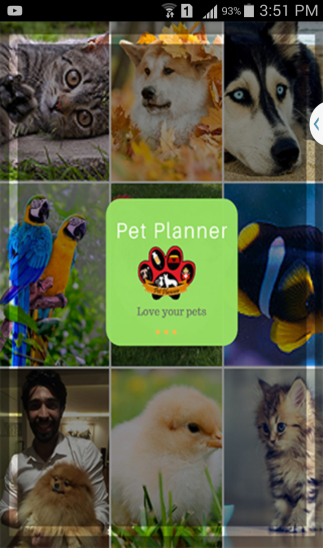
\includegraphics{00}
    \caption{Splash Screen}
\end{figure}

\newpage
\subsection{Login}

\begin{figure}[H]  
  \centering
    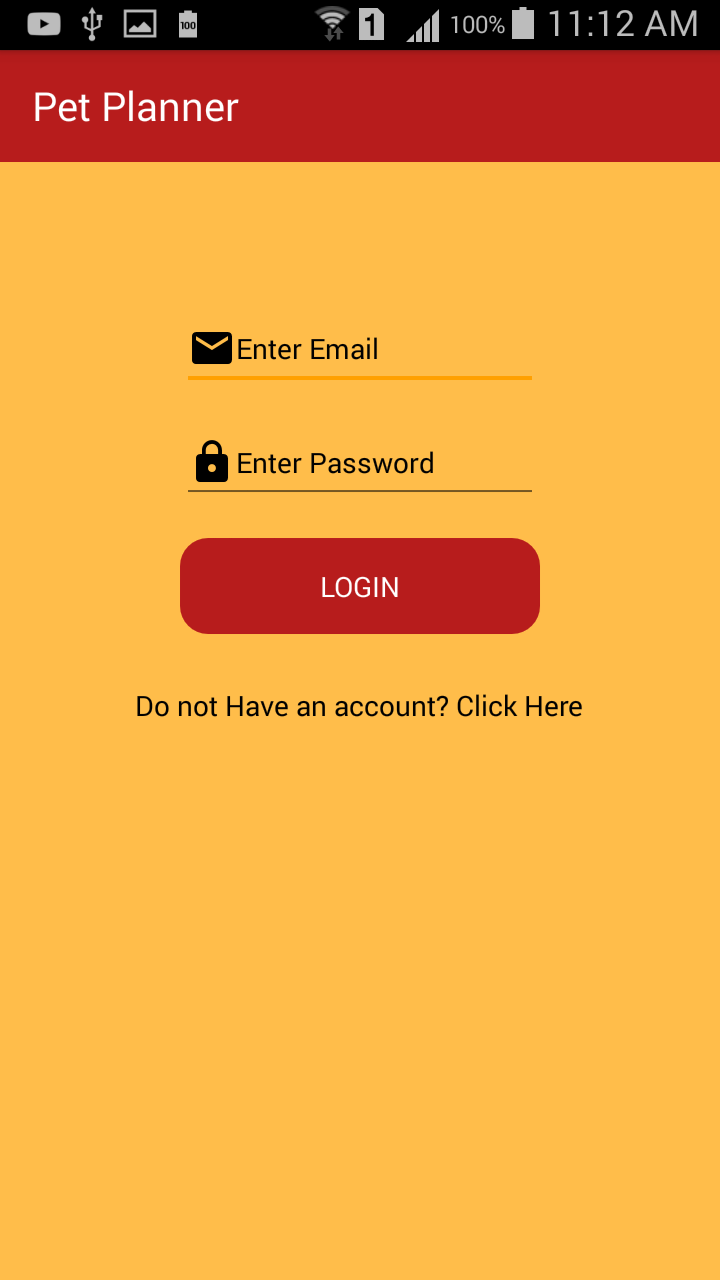
\includegraphics[scale=0.3]{81login}
    \caption{Login}
\end{figure}

User will enter valid email and password to login into the application.

\newpage
\subsection{Registration}
\begin{figure}[H]
  \centering
    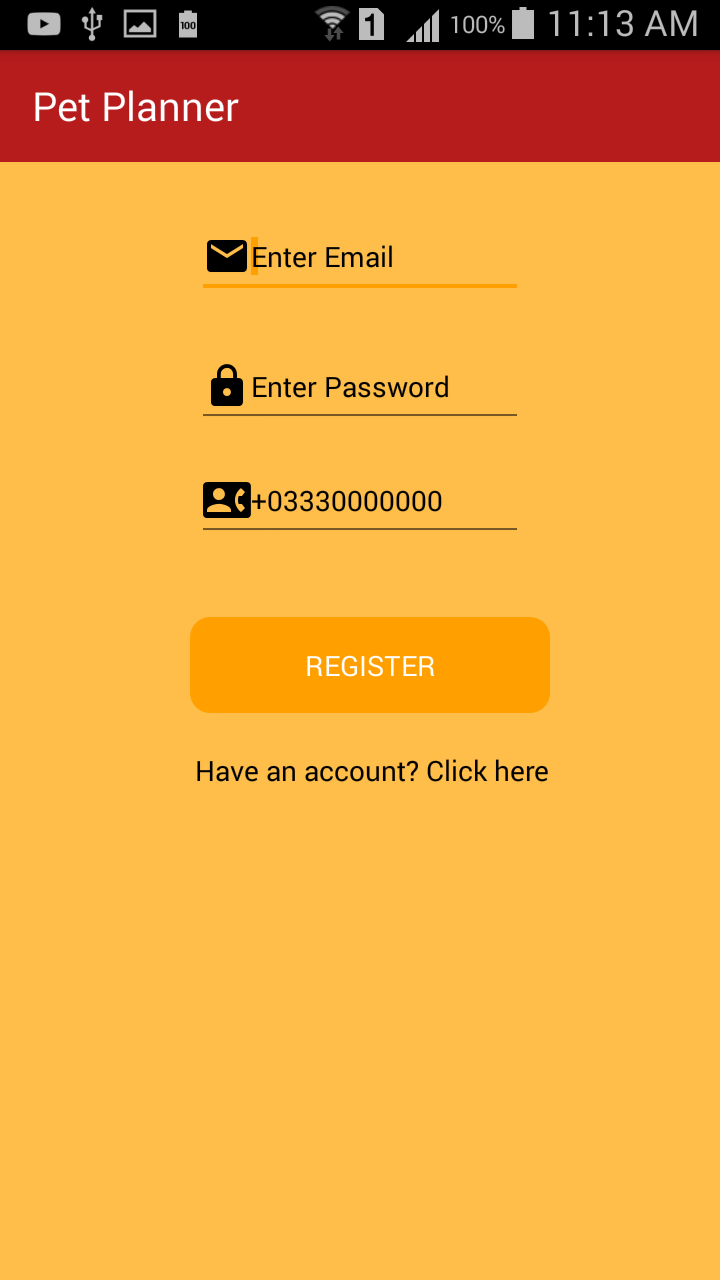
\includegraphics[scale=0.3]{82Registration}
     \caption{Registration}
\end{figure}

If user is new then he/she will register into the system.


\newpage
\subsection{Home Page}
\begin{figure}[H] 
  \centering
    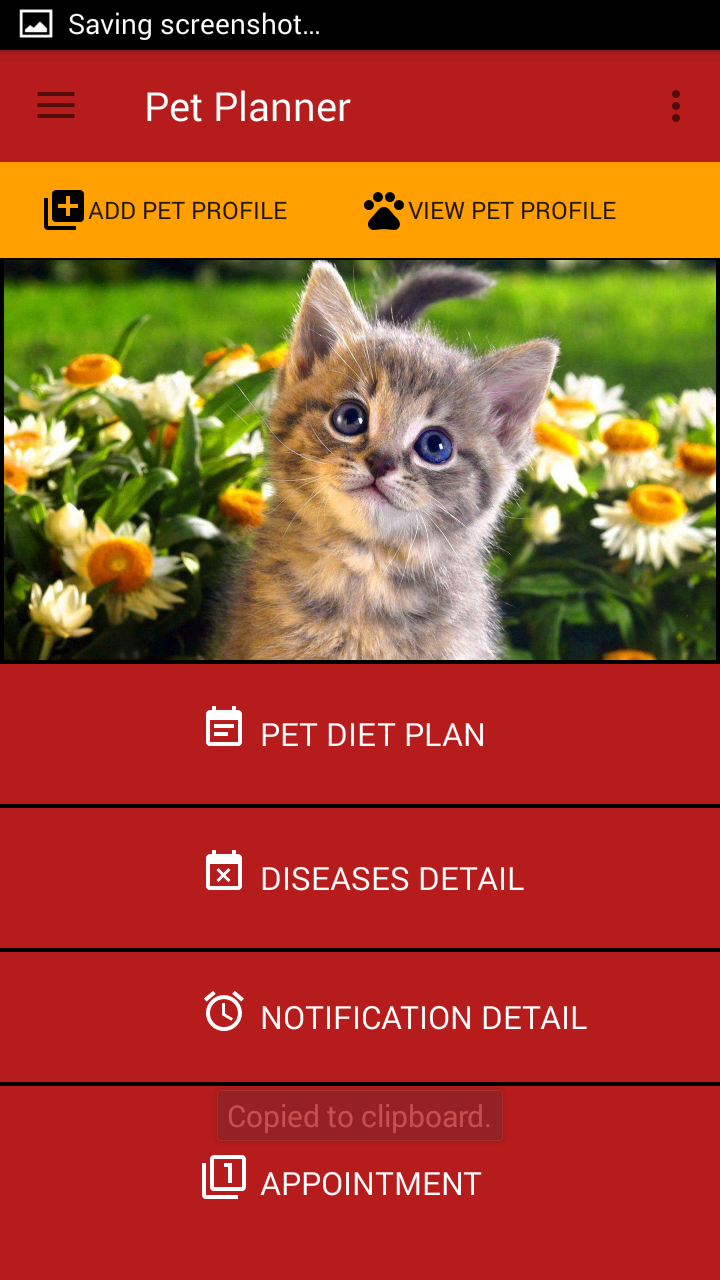
\includegraphics[scale=0.3]{89HomePage}
     \caption{Home Page}
\end{figure}
After the successful login user is able to add pet profile, view pet
 Profile, generate diet plan, view diseases details, generate alarm notifications and take appointment

\newpage
\subsection{Diet Plan}
\begin{figure}[H]
  \centering
    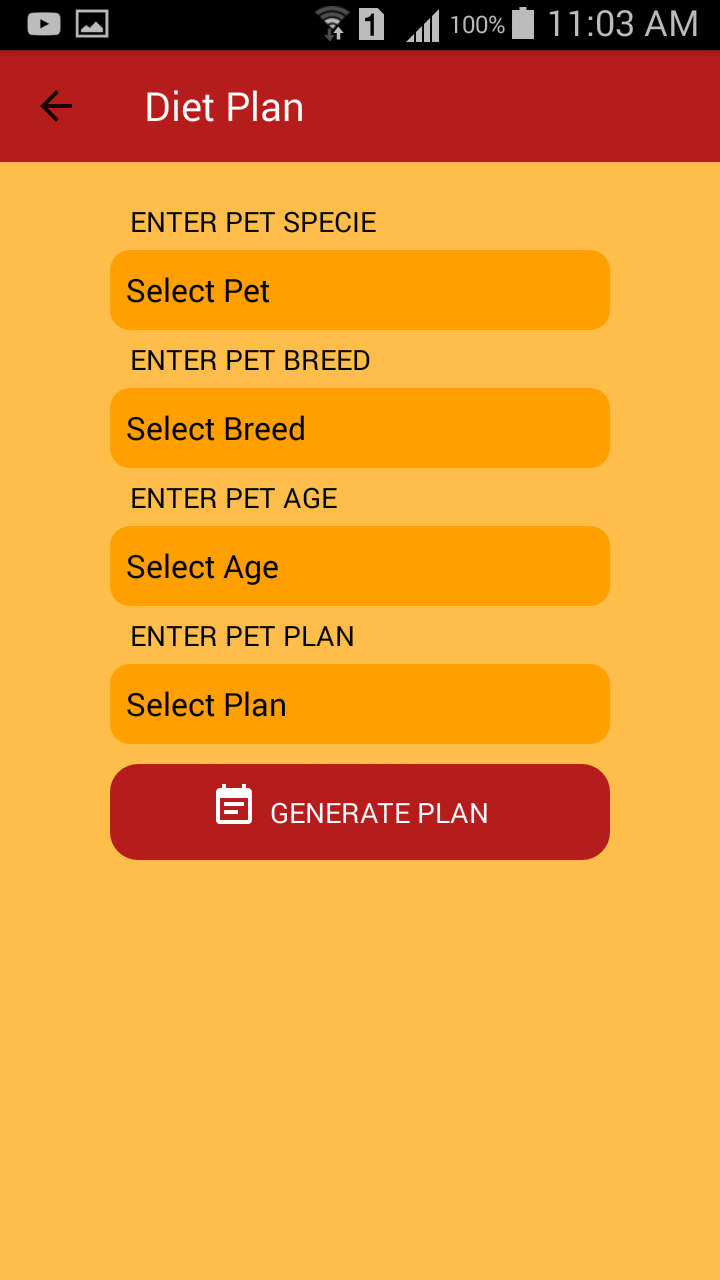
\includegraphics[scale=0.3]{86GenerateDietplan}
     \caption{Diet Plan}
\end{figure}

User can select pet specie, breed, age and plan to generate and download diet plan. 

\newpage
\subsection{Diseases Details}
\begin{figure}[H]
  \centering
    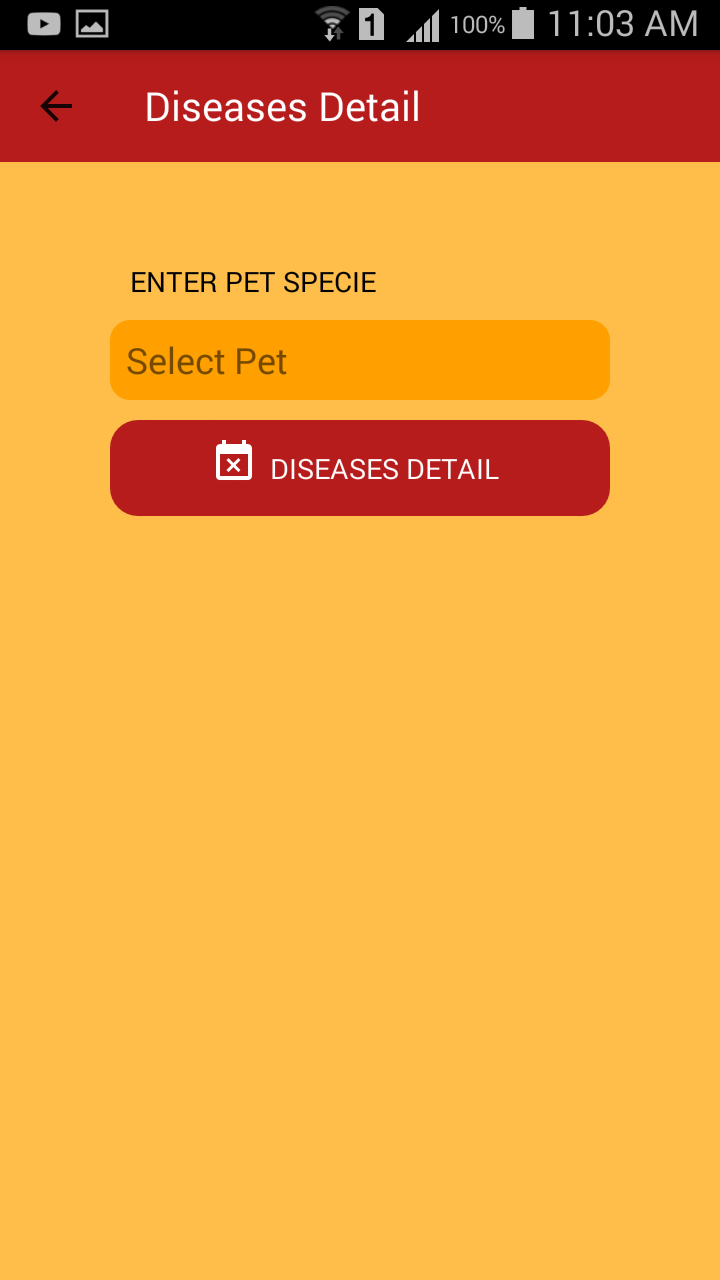
\includegraphics[scale=0.3]{87Diseases_Details}
     \caption{Diseases Details}
\end{figure}
User can select pet specie to view pet diseases details.

\newpage
\subsection{Notification Details}
\begin{figure}[H] 
  \centering
    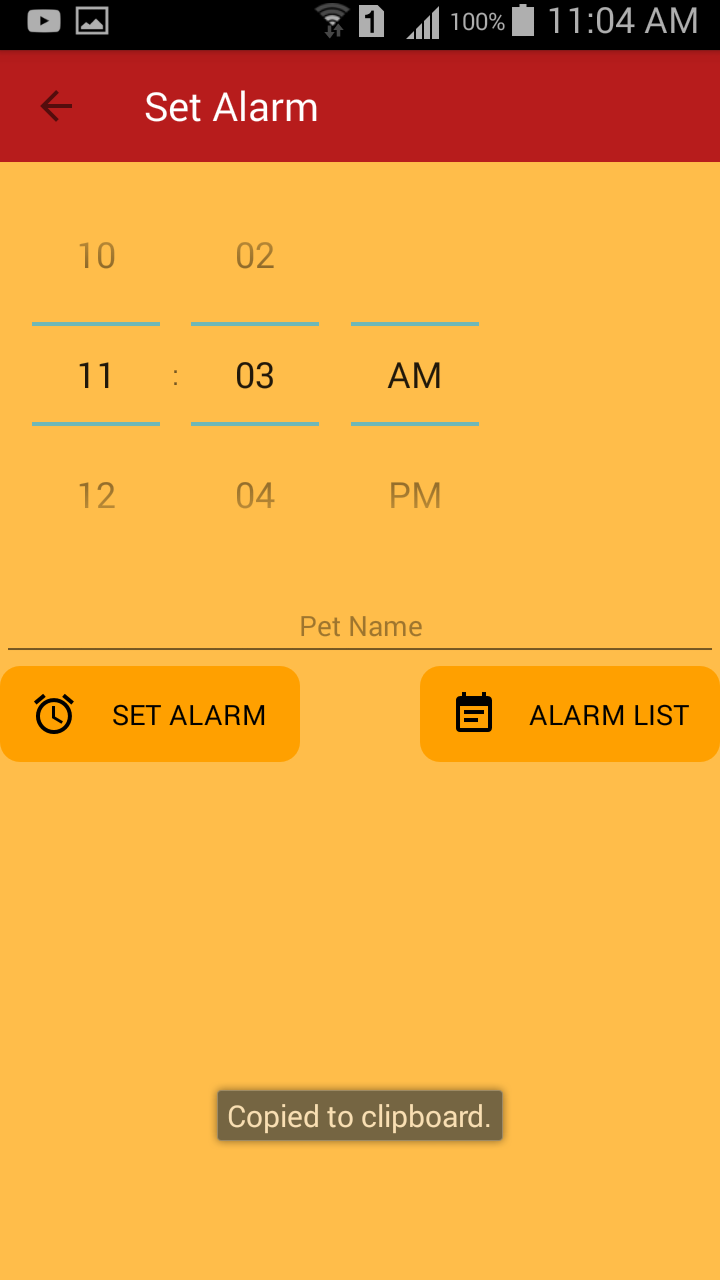
\includegraphics[scale=0.3]{85Alarmnotification}
    \caption{Notification Details}
\end{figure}

User can set alarm so that his pet could be feed.
\newpage
\subsection{Appointment}
\begin{figure}[H] 
  \centering
    
\includegraphics[scale=0.3]{88Appoint}
    \caption{Appointment}
\end{figure}

User can take appointment by clicking on Appoint button.
\newpage
\subsection{Add Pet Profile}
\begin{figure}[H] 
  \centering
    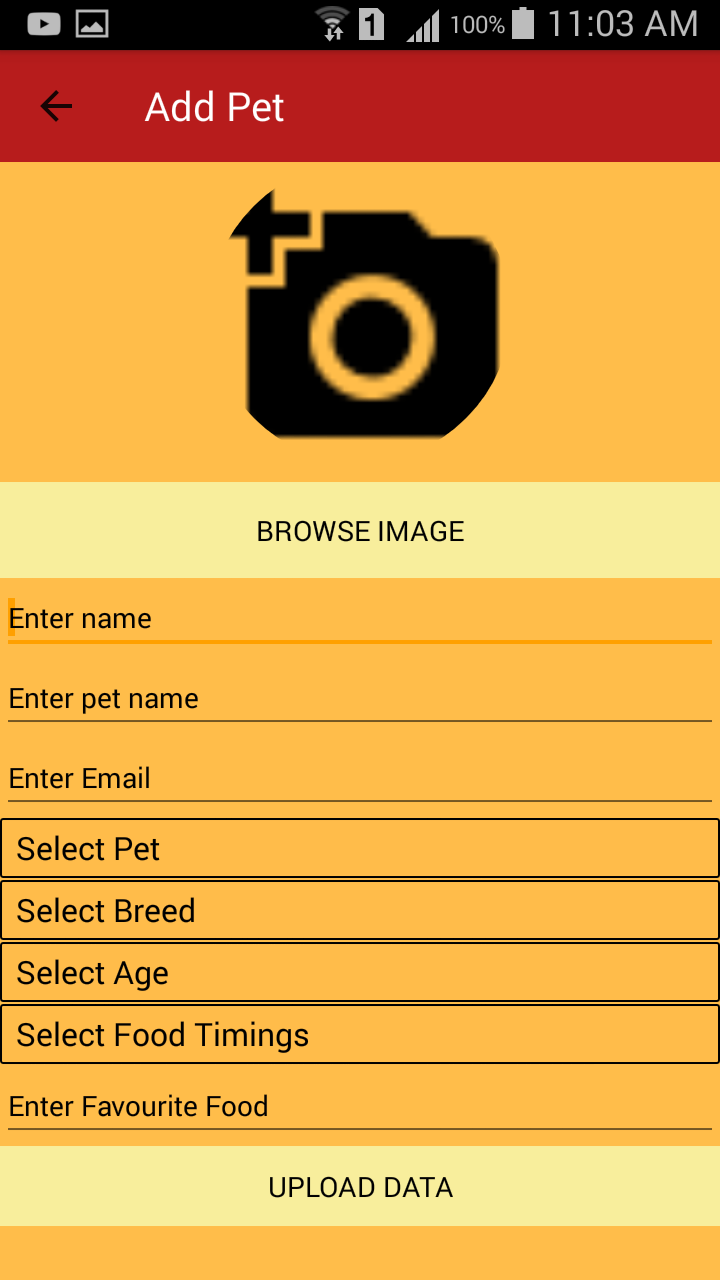
\includegraphics[scale=0.3]{83addpetprofile}
     \caption{Add Pet Profile}
\end{figure}
User can add pet details by filling all the fields.


\newpage
\subsection{View Pet Profile}

\begin{figure}[H]
  \centering
    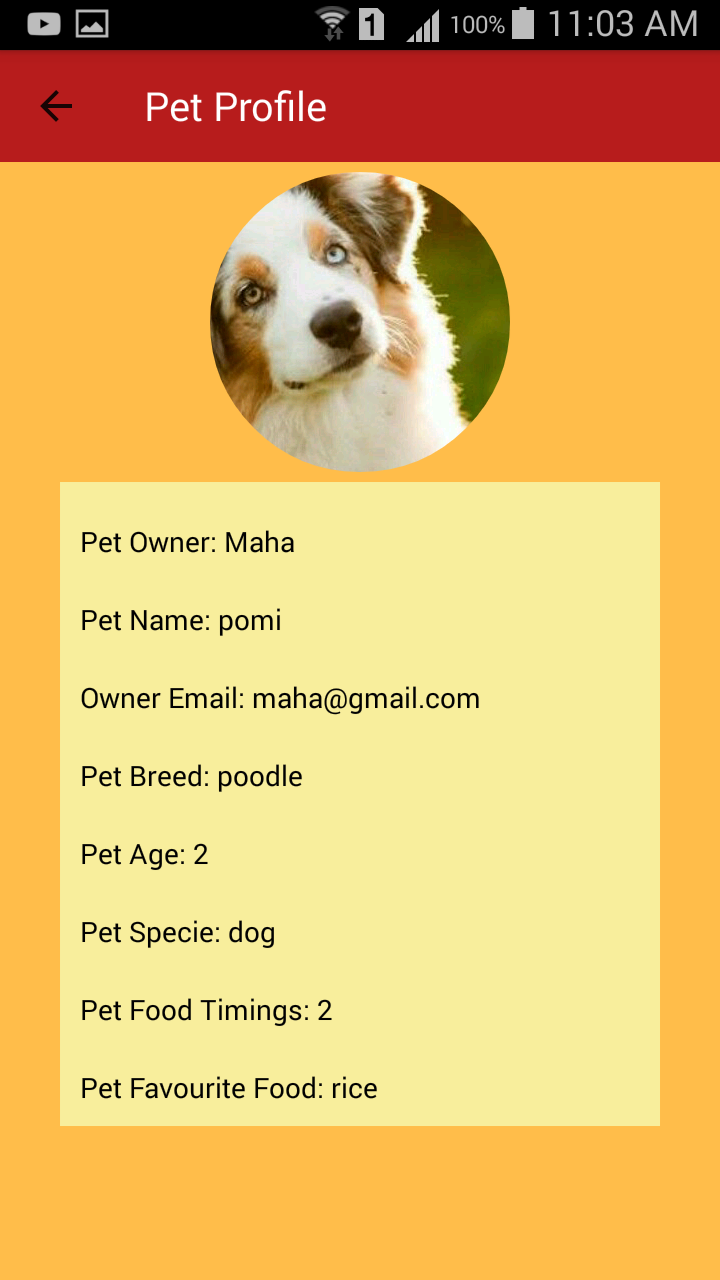
\includegraphics[scale=0.3]{84viewpetprofile}
      \caption{View Pet Profile}
\end{figure}

By clicking on view pet profile user is able to view pet profile.

\newpage
\subsection{Add as a Doctor}
\begin{figure}[H]
  \centering
    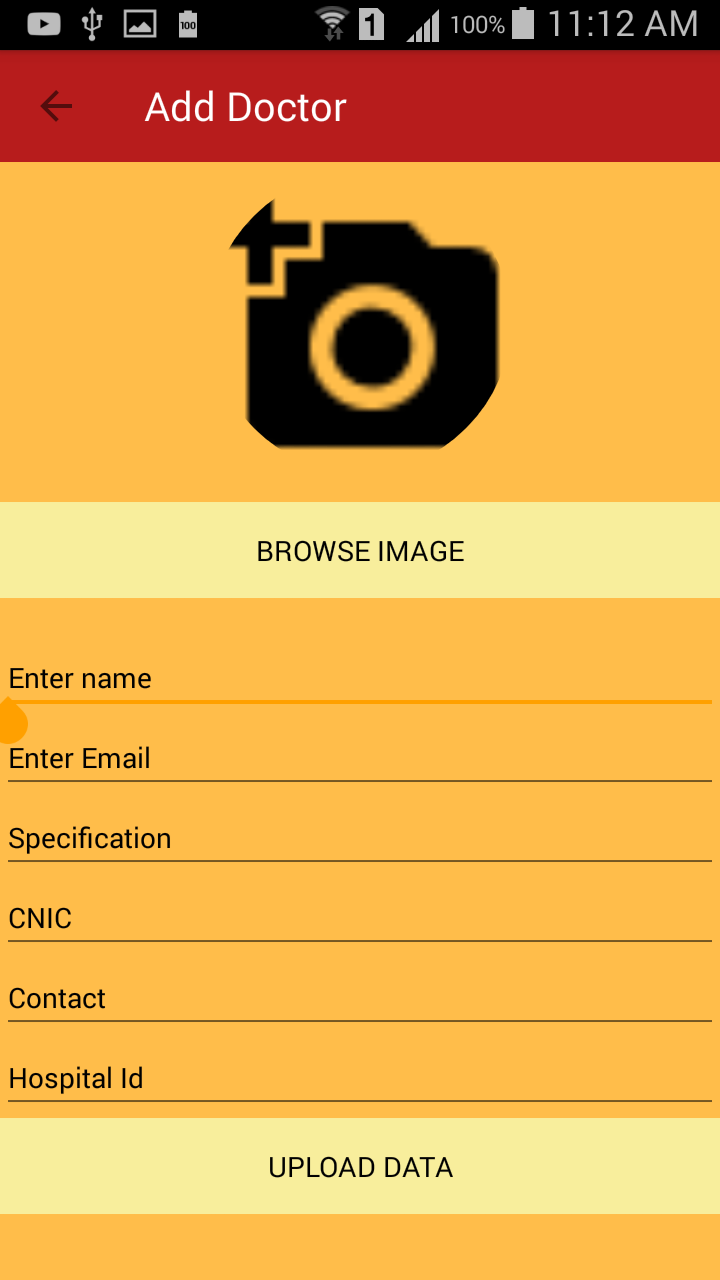
\includegraphics[scale=0.3]{90AddDoctorprofile}
      \caption{Add as a Doctor}
\end{figure}
Admin can be a doctor so he can register doctors by entering the correct hospital id assigned by the hospital to the doctor.

